% Options for packages loaded elsewhere
\PassOptionsToPackage{unicode}{hyperref}
\PassOptionsToPackage{hyphens}{url}
% !TeX program = pdfLaTeX
\documentclass[12pt]{article}
\usepackage{amsmath}
\usepackage{graphicx,psfrag,epsf}
\usepackage{enumerate}
\usepackage[]{natbib}
\usepackage{textcomp}


%\pdfminorversion=4
% NOTE: To produce blinded version, replace "0" with "1" below.
\newcommand{\blind}{0}

% DON'T change margins - should be 1 inch all around.
\addtolength{\oddsidemargin}{-.5in}%
\addtolength{\evensidemargin}{-1in}%
\addtolength{\textwidth}{1in}%
\addtolength{\textheight}{1.7in}%
\addtolength{\topmargin}{-1in}%

%% load any required packages here



% tightlist command for lists without linebreak
\providecommand{\tightlist}{%
  \setlength{\itemsep}{0pt}\setlength{\parskip}{0pt}}



\usepackage[dvipsnames]{xcolor} % colors
\newcommand{\ear}[1]{{\textcolor{blue}{#1}}}
\newcommand{\svp}[1]{{\textcolor{RedOrange}{#1}}}
\newcommand{\rh}[1]{{\textcolor{Green}{#1}}}
\newcommand\pcref[1]{(\cref{#1})}
\usepackage{algorithm,algpseudocode,booktabs}
\usepackage{hyperref}
\usepackage[capitalise]{cleveref}

\IfFileExists{bookmark.sty}{\usepackage{bookmark}}{\usepackage{hyperref}}
\IfFileExists{xurl.sty}{\usepackage{xurl}}{} % add URL line breaks if available
\hypersetup{
  pdftitle={Perception and Cognitive Implications of Logarithmic Scales for Exponentially Increasing Data: Perceptual Sensitivity Tested with Statistical Lineups},
  pdfkeywords={log scales, visual inference, graphical testing},
  hidelinks,
  pdfcreator={LaTeX via pandoc}}



\begin{document}


\def\spacingset#1{\renewcommand{\baselinestretch}%
{#1}\small\normalsize} \spacingset{1}


%%%%%%%%%%%%%%%%%%%%%%%%%%%%%%%%%%%%%%%%%%%%%%%%%%%%%%%%%%%%%%%%%%%%%%%%%%%%%%

\if0\blind
{
  \title{\bf Perception and Cognitive Implications of Logarithmic Scales
for Exponentially Increasing Data: Perceptual Sensitivity Tested with
Statistical Lineups}

  \author{
        Emily A. Robinson 1 \\
    Department of Statistics, California Polytechnic State University -
San Luis Obispo\\
     and \\     Reka Howard 2 \\
    Department of Statistics, University of Nebraska - Lincoln\\
     and \\     Susan VanderPlas 3 \\
    Department of Statistics, University of Nebraska - Lincoln\\
      }
  \maketitle
} \fi

\if1\blind
{
  \bigskip
  \bigskip
  \bigskip
  \begin{center}
    {\LARGE\bf Perception and Cognitive Implications of Logarithmic
Scales for Exponentially Increasing Data: Perceptual Sensitivity Tested
with Statistical Lineups}
  \end{center}
  \medskip
} \fi

\bigskip
\begin{abstract}
Logarithmic transformations are a standard solution to displaying data
that span several magnitudes within a single graph. This paper
investigates the impact of log scales on perceptual sensitivity through
a visual inference experiment using statistical lineups. Our study
evaluated participant's ability to detect differences between
exponentially increasing data, characterized by varying levels of
curvature, using both linear and logarithmic scales. Participants were
presented with a series of plots and asked to identify the panel that
appeared most different from the others. Due to the choice of scale
altering the contextual appearance of the data, the results revealed
slight perceptual advantages for both scales depending on the curvatures
of the compared data. This study serves as the initial part of a
three-paper series dedicated to understanding the perceptual and
cognitive implications of using logarithmic scales for visualizing
exponentially increasing data. These studies serve as an example of
multi-modal graphical testing, examining different levels of engagement
and interaction with graphics to establish nuanced and specific
guidelines for graphical design.
\end{abstract}

\noindent%
{\it Keywords:} log scales, visual inference, graphical testing

\vfill

\newpage
\spacingset{1.9} % DON'T change the spacing!

\hypertarget{introduction}{%
\section{Introduction}\label{introduction}}

Effective communication of data is critical in influencing people's
opinions and actions. This consideration was particularly true during
the COVID-19 pandemic, where data visualizations and dashboards were
vital in informing the public and policymakers about the outbreak's
status. Local governments relied on graphics to inform their decisions
about shutdowns and mask mandates, while residents were presented with
data visualizations to encourage compliance with these regulations. A
major issue designers encountered when creating COVID-19 plots was how
to display data from a wide range of values
\citep[\citet{burnmurdoch_2020}]{fagen-ulmschneider_2020}. When faced
with data that span several orders of magnitude, we must decide whether
to show the data on its original scale (compressing the smaller
magnitudes into a relatively small area) or to transform the scale and
alter the contextual appearance of the data. Log axis transformations
have emerged as a standard solution to this challenge, as they allow for
the display of data over several orders of magnitude within a single
graph.

Exponential data is one such example of a function that compresses
smaller magnitudes into a smaller area; \cref{fig:log-scales} presents
hard drive capacity over the past forty years on both the linear and log
scales to demonstrate the usefulness of log scales when dealing with
data spanning multiple magnitudes. Logarithms facilitate the conversion
of multiplicative relationships (displaying 1 \& 10 with a distance of
10 units apart and displaying 10 \& 100 with a distance of 90 units
apart) to additive relationships (displaying 1 \& 10 and 10 \& 100 an
equal distance apart), highlighting proportional relationships and
linearizing power functions \citep{menge_logarithmic_2018}. Logarithms
also have practical applications, simplifying the computation of small
numbers such as likelihoods and transforming data to conform to
statistical assumptions. Although log scales have a long history of use
in fields such as ecology, psychophysics, engineering, and physics
\citep{heckler_student_2013, waddell2005comparisons}, there is still a
need to understand the implications of their use and provide best
practices for their implementation.

\begin{figure}[tbp]

{\centering 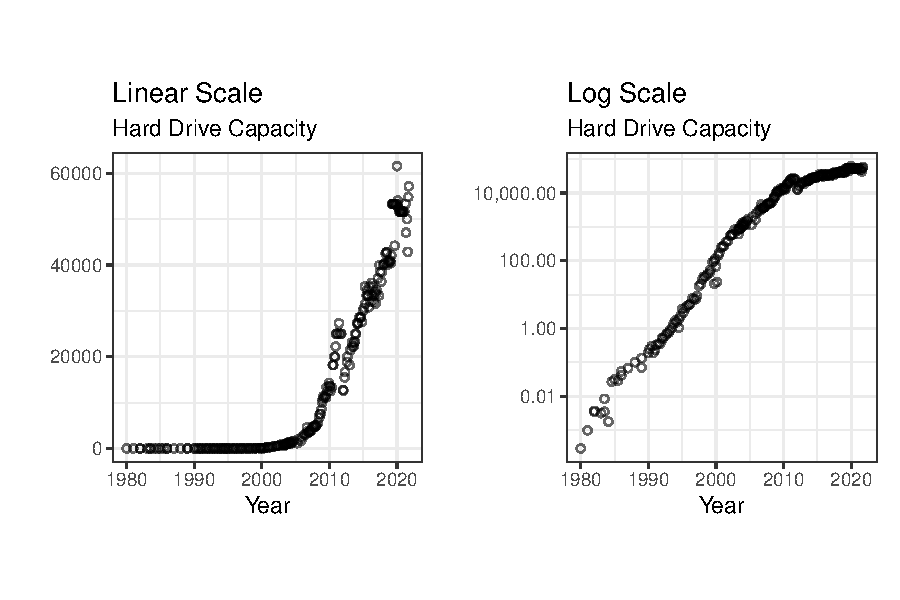
\includegraphics[width=1\linewidth,]{updated-ASA-template_files/figure-latex/log-scales-1} 

}

\caption{These plots present hard drive capacity over the past forty years on both the linear and log scale and illustrate the use of the log scale when displaying data which spans several magnitudes.}\label{fig:log-scales}
\end{figure}

Apart from the biases resulting from using log scales, there is a
general misinterpretation of exponential growth. Early stages of
exponential growth often appear to have a small growth rate, while the
middle stage seems to exhibit more quadratic growth. It is only in the
later stages that the exponential growth becomes apparent.
\cref{fig:exponential-stages} highlights the three stages and associated
appearances of exponential growth at each stage
\citep{vonbergmann_2021}. This misinterpretation can lead to decisions
made under inaccurate understanding, resulting in potential
consequences.

\begin{figure}[tbp]

{\centering 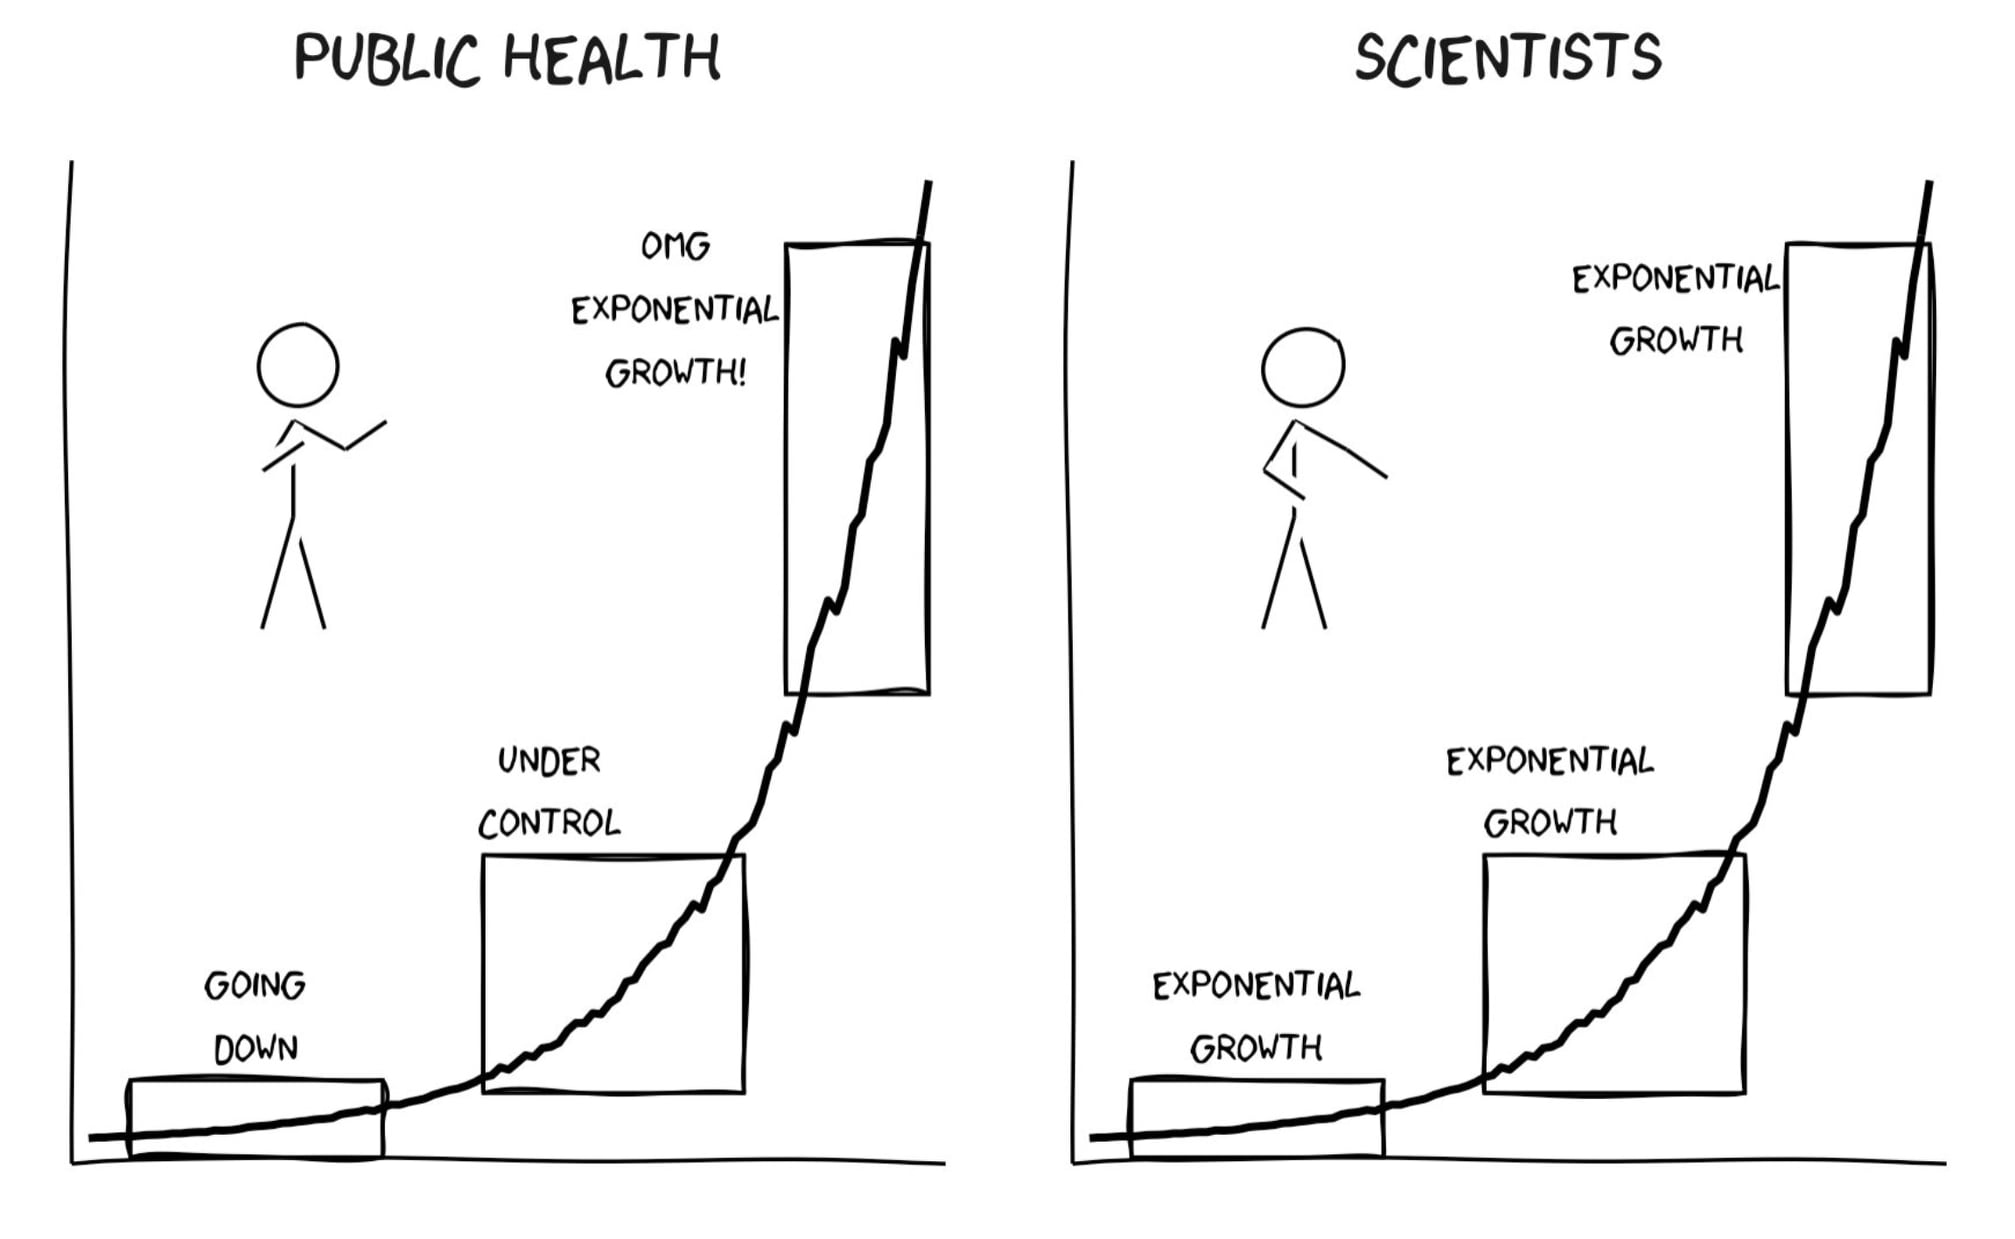
\includegraphics[width=1\linewidth,]{images/exponential-stages-comic} 

}

\caption{This figure highlights the three stages and associated appearances of exponential growth at each stage. Early stages of exponential growth often appear to have a small growth rate, while the middle stage seems to exhibit more quadratic growth. It is only in the later stages that the exponential growth becomes apparent.}\label{fig:exponential-stages}
\end{figure}

Previous studies have explored the estimation and prediction of
exponential growth and found that individuals often underestimate
exponential growth when presented values numerically and graphically
\citep{wagenaar_misperception_1975}. The hierarchy of plot objects, such
as lengths and angles, as described by \citet{cleveland_graphical_1985},
offers a possible explanation for the underestimation observed in
exponentially increasing trends. Experiments conducted by
\citet{wagenaar_misperception_1975}, \citet{jones_polynomial_1977}, and
\citet{mackinnon_feedback_1991} aimed to improve estimation accuracy for
exponential growth. While contextual knowledge or experience did not
enhance estimation, instruction on exponential growth reduced
underestimation by prompting participants to adjust their initial
starting value
\citep{wagenaar_misperception_1975, jones_polynomial_1977}. Furthermore,
providing immediate feedback to participants about the accuracy of their
predictions improved estimation \citep{mackinnon_feedback_1991}.

Log transforming the data may address our inability to predict
exponential growth accurately. However, this transformation introduces
new complexities, as most readers may need to be mathematically
sophisticated enough to intuitively understand logarithmic math and
translate it back into real-world effects. Despite the transformative
power of logarithmic scales in facilitating accurate data
representation, \citet{menge_logarithmic_2018}'s survey of ecologists
highlights the challenges associated with the widespread comprehension
of log-scaled data. Notably, the study identifies prevalent
misconceptions arising from linear extrapolation assumptions in log-log
space, a factor that often leads to neglect of the underlying
exponential relationships in linear-linear space.

Building upon the need for a nuanced understanding of data
representation, \citet{buja_statistical_2009} introduced statistical
lineups as a framework for statistical inference and graphical tests.
Statistical lineups treat a data plot as a visual statistic, summarizing
the data as a numerical function or mapping. Evaluation of a panel in a
statistical lineup requires visual inspection by a person, and if visual
evaluations lead to different results, two visualization methods are
deemed significantly different. Recent studies have utilized statistical
lineups to quantify the perception of graphical design choices
\citep{hofmann_graphical_2012, loy_model_2017, loy_variations_2016, vanderplas_clusters_2017}.
Statistical lineups provide an elegant way of combining perception and
statistical hypothesis testing through graphical experiments
\citep{majumder_validation_2013, vanderplas_testing_2020, wickham2010graphical}.

The term `lineup' is an analogy to police lineups in criminal
investigations, where witnesses identify the criminal from a group of
individuals. Similarly, researchers present a statistical lineup plot
consisting of smaller panels and ask the viewer to identify the panel
that contains the actual data from a set of decoy null plots.
Researchers generate null plots containing data generated according to a
prespecified hypothesis using permutation or simulation. Typically, a
statistical lineup consists of 20 panels, with one target panel and 19
null panels. If the viewer can identify the target panel from the null
panels, it suggests that the actual data is visually distinct from the
data generated under the null model.

While explicit graphical tests direct the participant to a specific
feature of a plot to answer a particular question, implicit graphical
tests require the user to identify both the purpose and function of the
plot in order to evaluate the plots shown. Furthermore, implicit
graphical tests, such as lineups, simultaneously test for multiple
visual features, including outliers, clusters, and linear and nonlinear
relationships \citep{vanderplas2015spatial}. Researchers can collect
responses from multiple viewers using crowd-sourcing websites such as
Prolific and Amazon Mechanical Turk.

In this paper, our primary focus is to evaluate the benefits and
drawbacks of using log scales, specifically delving into their impact on
perceptual sensitivity towards the degree of curvature. To address this,
we conducted a visual inference experiment employing statistical lineups
\citep{buja_statistical_2009}. Although our findings could have broad
applications to various functions resulting in curvature, our experiment
deliberately centered on participants' ability to identify differences
in the curvature of exponentially increasing curves when presented with
both linear and log scales. We discuss the nuances and challenges of
testing the perception of exponential growth in the appendix.
Importantly, this investigation did not necessitate participants to
undergo mathematical training or possess a prior understanding of
exponential growth or logarithmic scales. Instead, it aimed to unravel
the inherent ability to identify differences in curvature within charts,
focusing on the fundamental nature of visual perception.

In \protect\hyperlink{methods}{Section 2} we describe the participant
sample, the graphical task, data generation process, and study design.
\protect\hyperlink{results}{Section 3} describes the participant data
collected and shares results from the statistical analyses of the data
using a generalized linear mixed model. We present overall conclusions
and discussion of the results in
\protect\hyperlink{conclusion-discussion}{Section 4}, and provide an
overview of future related papers. The
\protect\hyperlink{supplementary-material}{Supplementary Material}
includes a link to the RShiny data collection applet, participant data
used for analysis, and code to replicate the analysis. The results of
this study lay the groundwork for further exploration of the
implications of using log scales in data visualization.

\hypertarget{methods}{%
\section{Study Development and Methods}\label{methods}}

\hypertarget{data-generation}{%
\subsection{Data Generation}\label{data-generation}}

In this study, we simulated data from an exponential model to generate
the target and null data sets; the models between panels differ in the
parameter values selected for the null and target panels. In order to
guarantee the simulated data spans the same domain and range of values
for each statistical lineup panel, we began with a domain constraint of
\(x\in [0,20]\) and a range constraint of \(y\in [10,100]\) with
\(N = 50\) points randomly assigned throughout the domain. We mapped the
randomly generated \(x\) values to a corresponding \(y\) value based on
an exponential model with predetermined parameter values and
multiplicative random errors to simulate the response. These constraints
assure that participants who select the target panel are doing so
because of their visual perception differentiating between curvature or
growth rate rather than different starting or ending values.

We simulated data based on a three-parameter exponential model with
multiplicative errors: \begin{align}
y_i & = \alpha\cdot e^{\beta\cdot x_i + \epsilon_i} + \theta \\
\text{with } \epsilon_i & \sim N(0, \sigma^2). \nonumber
\end{align} The parameters \(\alpha\) and \(\theta\) were adjusted based
on \(\beta\) and \(\sigma^2\) to guarantee the range and domain
constraints are met. The model generated \(N = 50\) points
\((x_i, y_i), i = 1,...,N\) where \(x\) and \(y\) have an increasing
exponential relationship. The heuristic data generation procedure is
described in \cref{alg:lineup-parameter-estimation-algorithm} and
\cref{alg:lineup-exponential-data-simulation-algorithm}.

\begin{algorithm}
  \caption{Lineup Parameter Estimation}\label{alg:lineup-parameter-estimation-algorithm}
  \begin{algorithmic}[1]
    \Statex \hspace*{-1em}\textbullet~\textbf{Input Parameters:} domain $x\in[0,20]$, range $y\in[10,100]$, midpoint $x_{mid}$.
    \Statex \hspace*{-1em}\textbullet~\textbf{Output Parameters:} estimated model parameters $\hat\alpha, \hat\beta, \hat\theta$.
    \State In order to obtain the two middle points (total of four points for estimating three parameters), determine the $y=-x$ line scaled to fit the assigned domain and range.
    \State Map the values $x_{mid} - 0.1$ and $x_{mid} + 0.1$ to the $y=-x$ line for the two additional points.
    \State From the set of points $(x_k, y_k)$ for $k = 1,2,3,4$, calculate the coefficients from the linear regression model $\ln(y_k) = b_0 +b_1x_k$ to obtain starting values for $\alpha_0 = e^{b_0}, \beta_0 =  b_1, \theta_0 = 0.5\cdot \min(y)$
    \State Using the \texttt{nls} function from the base \texttt{stats} package in Rstudio [@Rstudio] and the starting parameter values - $\alpha_0, \beta_0, \theta_0$ - fit the nonlinear model, $y_k = \alpha\cdot e^{\beta\cdot x_k}+\theta$ to get estimated parameter values for $\hat\alpha, \hat\beta, \hat\theta.$
  \end{algorithmic}
\end{algorithm}

\begin{algorithm}
  \caption{Lineup Exponential Data Simulation}\label{alg:lineup-exponential-data-simulation-algorithm}
  \begin{algorithmic}[1]
    \Statex \hspace*{-1em}\textbullet~\textbf{Input Parameters:} sample size $N = 50$, estimated parameters $\hat\alpha$, $\hat\beta$, and $\hat\theta$, from \cref{alg:lineup-parameter-estimation-algorithm}, and standard deviation $\sigma$ from the exponential curve.
    \Statex \hspace*{-1em}\textbullet~\textbf{Output Parameters:} $N$ points, in the form of vectors $\mathbf{x}$ and $\mathbf{y}$.
    \State Generate $\tilde x_j, j = 1,..., \frac{3}{4}N$ as a sequence of evenly spaced points in $[0,20]$. This ensures the full domain of $x$ is used, fulfilling the constraints of spanning the same domain and range for each parameter combination.
    \State Obtain $\tilde x_i, i = 1,...,N$ by sampling $N = 50$ values from the set of $\tilde x_j$ values. This guarantees some variability and potential clustering in the exponential growth curve disrupting the perception due to continuity of points.
    \State Obtain the final $x_i$ values by jittering $\tilde x_i$.
    \State Calculate $\tilde\alpha = \frac{\hat\alpha}{e^{\sigma^2/2}}.$ This ensures that the range of simulated values for different standard deviation parameters has an equal expected value for a given rate of change due to the non-constant variance across the domain.
    \State Generate $y_i = \tilde\alpha\cdot e^{\hat\beta x_i + e_i}+\hat\theta$ where $e_i\sim N(0,\sigma^2).$
  \end{algorithmic}
\end{algorithm}

\hypertarget{lineups-parameter-selection}{%
\subsection{Parameter Selection}\label{lineups-parameter-selection}}

We chose three levels of trend curvature (low curvature, medium
curvature, and high curvature). For each curvature level, we simulated
1,000 data sets of \((x_{ij}, y_{ij})\) points for \(i = 1,...,50\)
increments of \(x\)-values and replicated \(j = 1,...,10\) corresponding
\(y\)-values per \(x\)-value. Each generated \(x_i\) point from
\cref{alg:lineup-exponential-data-simulation-algorithm} was replicated
ten times. We fit a linear regression model on each of the individual
data sets and computed the lack of fit statistic (LOF) which measures
the deviation of the data from the linear regression model. After
obtaining the LOF statistic for each level of curvature, we evaluated
the density plots (\cref{fig:lof-density-curves}) to provide a metric
for differentiating between the curvature levels and thus detecting the
target plot. While the LOF statistic provides a numerical value for
discriminating between the difficulty levels, it cannot be directly
related to the perceptual discriminability; it serves primarily as an
approximation to ensure that we are testing parameters at several
distinct curvature levels. \cref{tab:parameter-data} lists the final
parameters used for data simulation.

\begin{figure}[tbp]

{\centering 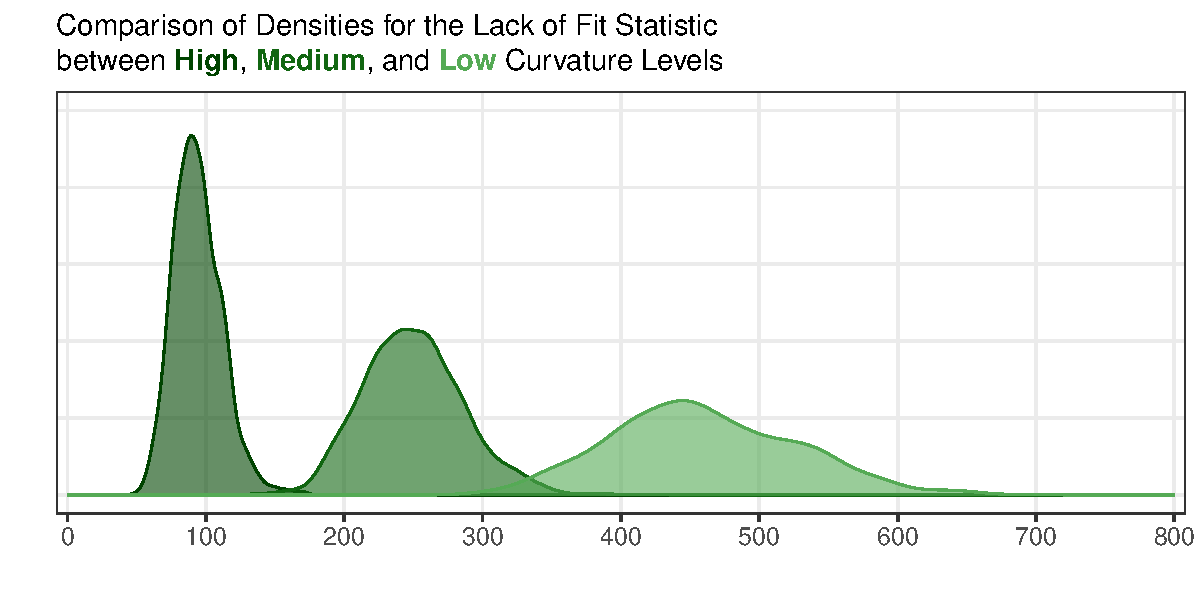
\includegraphics[width=1\linewidth,]{updated-ASA-template_files/figure-latex/lof-density-curves-1} 

}

\caption{Density plot of the lack of fit statistic showing separation of difficulty levels: obvious curvature, noticable curvature, and almost linear.}\label{fig:lof-density-curves}
\end{figure}

\begin{table}

\caption{\label{tab:parameter-data}Lineup data simulation final parameters}
\centering
\begin{tabular}[t]{lrrrrrr}
\toprule
Curvature Level & $x_{mid}$ & $\hat\alpha$ & $\tilde\alpha$ & $\hat\beta$ & $\hat\theta$ & $\hat\sigma$\\
\midrule
High & 14.5 & 0.91 & 0.88 & 0.23 & 9.10 & 0.25\\
Medium & 13.0 & 6.86 & 6.82 & 0.13 & 3.14 & 0.12\\
Low & 11.5 & 37.26 & 37.22 & 0.06 & -27.26 & 0.05\\
\bottomrule
\end{tabular}
\end{table}

\hypertarget{lineup-setup}{%
\subsection{Lineup Setup}\label{lineup-setup}}

To generate the small multiple scatter plots for the statistical lineups
shown to participants in the study, we simulated a single data set
corresponding to curvature level A for the target plot and multiple data
sets corresponding to curvature level B for the null plots. The
\texttt{nullabor} package in R \citep{buja_statistical_2009} randomly
assigned the target plot to one of the panels surrounded by panels
containing null plots. The target and null panels span a similar domain
and range due to the implemented constraints when simulating the data;
the rationale for this decision is based on preattentive feature
perception \citep{wolfe2019preattentive} and is discussed in detail in
the appendix.

There were a total of six lineup curvature combinations;
\cref{fig:curvature-combination-example} illustrates the six lineup
curvature combinations (top: linear scale; bottom: log scale) where the
solid line indicates the curvature level designated to the target plot
while the dashed line indicates the curvature level assigned to the null
plots. Two sets of each lineup curvature combination were simulated (a
total of twelve test data sets) and plotted on both the linear scale and
the log scale (24 test lineup plots). In addition, three curvature
combinations generated homogeneous ``Rorschach'' lineups, where all
panels were from the same distribution. Each participant evaluated one
``Rorschach'' lineup. Results from the ``Rorschach'' evaluations
indicate null panel selections were distributed relatively evenly with
multiple candidates for the most interesting panel. We display and
further discuss the ``Rorschach'' evaluation results in the appendix.

\begin{figure}[tbp]

{\centering 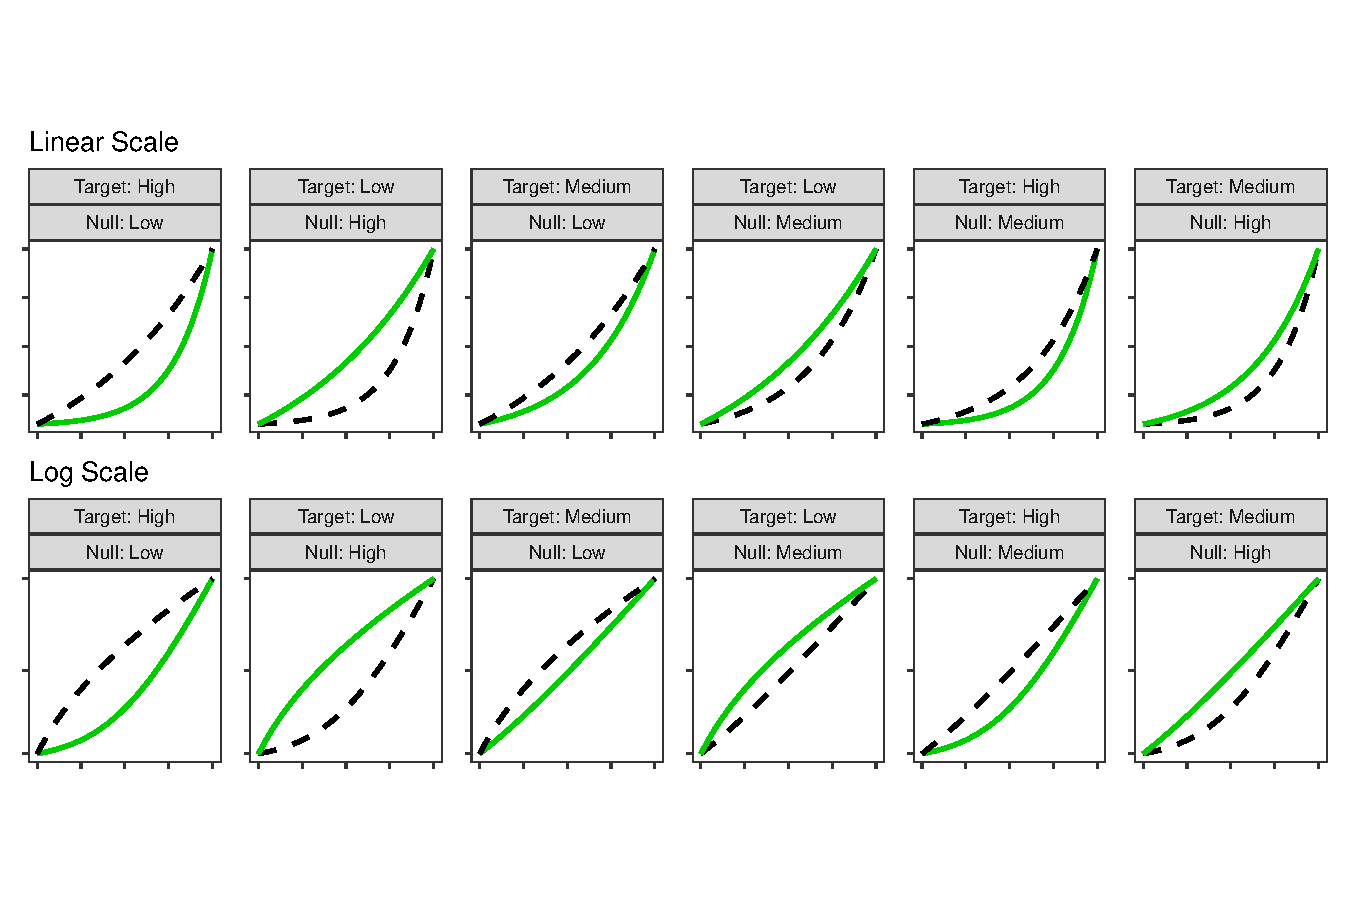
\includegraphics[width=1\linewidth,]{updated-ASA-template_files/figure-latex/curvature-combination-example-1} 

}

\caption{Thumbnail plots illustrating the six curvature combinations displayed on both scales (linear and log). The solid line indicates the curvature level to be identified as the target plot from amongst a set of null plots with the curvature level indicated by the dashed line.}\label{fig:curvature-combination-example}
\end{figure}

\cref{fig:lineup-example} presents examples of statistical lineups with
the target data simulated with exponential parameters corresponding high
curvature and the surrounding null panels simulated with parameters for
low curvature. The statistical lineup on the left presents increasing
exponential data with displayed on a linear scale with panel 13 as the
target panel. The lineup on the right shows increasing exponential data
plotted on a log scale with panel 4 as the target panel.

\begin{figure}[tbp]

{\centering 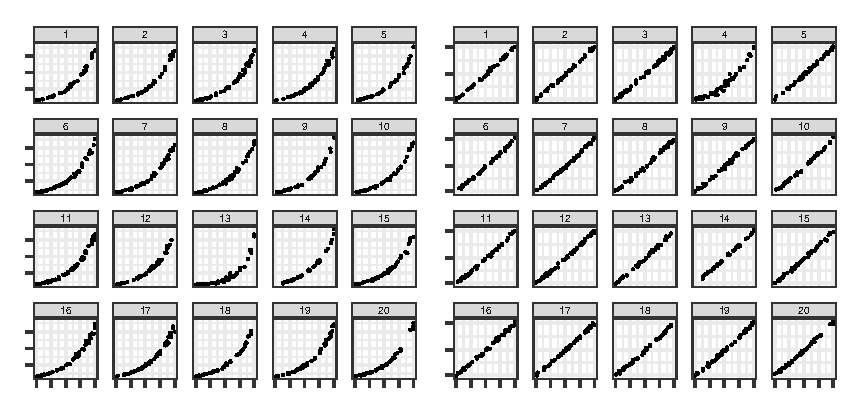
\includegraphics[width=\linewidth,]{updated-ASA-template_files/figure-latex/lineup-example-1} 

}

\caption{The lineup plot on the left displays increasing exponential data on a linear scale with panel (13 as the target. The lineup plot on the right displays increasing exponential data on the log scale with panel 4 as the target.}\label{fig:lineup-example}
\end{figure}

\bibliographystyle{apalike}
\bibliography{bibliography.bib}



\end{document}
